% Updated LaTeX figure references for the 6 new figures
% Place these in your paper where appropriate

% ============================================================================
% MAIN PAPER FIGURES
% ============================================================================

% PLACEMENT: Insert after Section 4.2 "Overall objective-extraction accuracy"
% This figure shows the main results and should appear right after discussing overall performance
\begin{figure}[t]
  \centering
  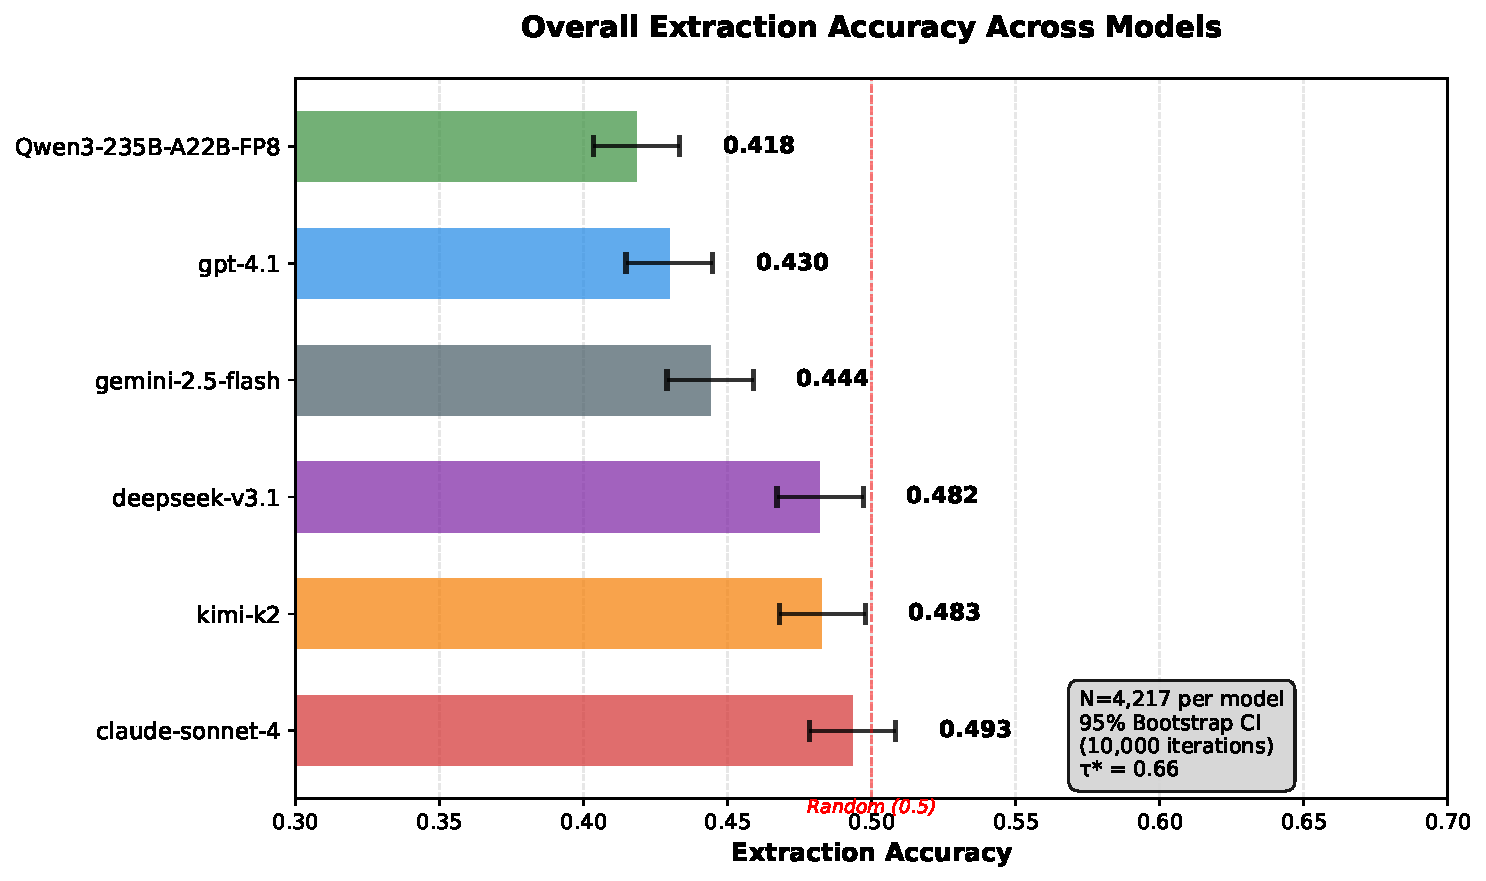
\includegraphics[width=0.7\linewidth]{fig_overall_accuracy.pdf}
  \caption{Overall objective-extraction accuracy with 95\% bootstrap confidence intervals (10,000 iterations) for six state-of-the-art models evaluated on $N{=}4,217$ instances each.}
  \label{fig:overall-acc}
\end{figure}

% PLACEMENT: Insert in Section 4.3 "Dataset-wise performance"
% This figure breaks down performance by dataset and should accompany the dataset analysis
\begin{figure}[t]
  \centering
  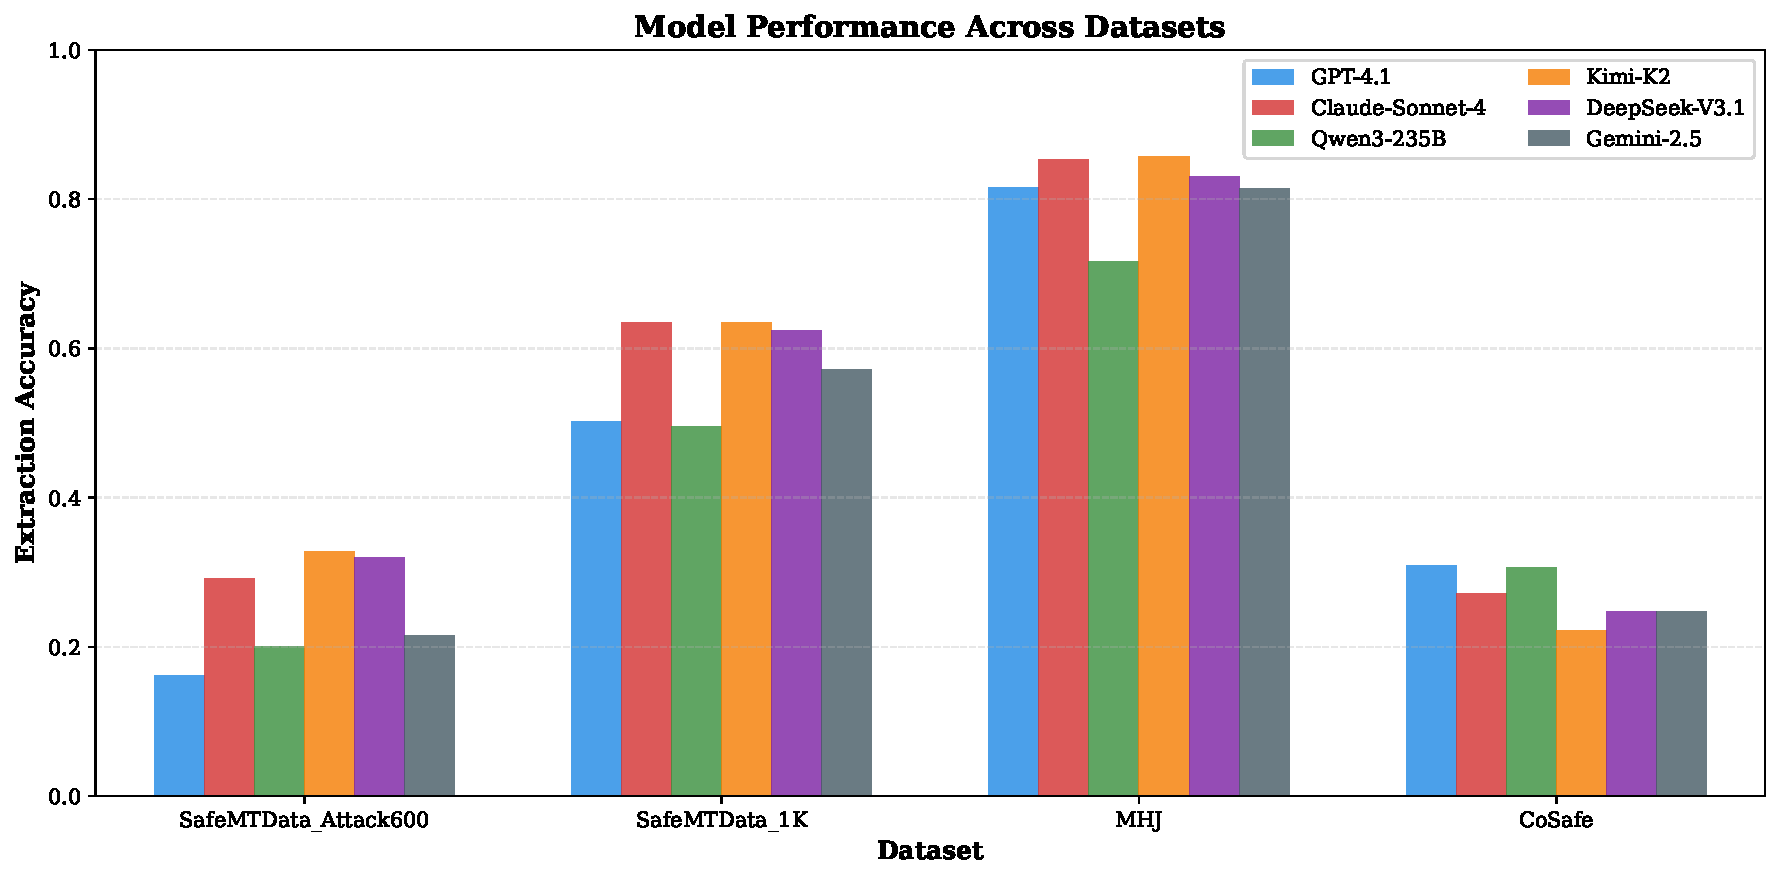
\includegraphics[width=\linewidth]{fig_per_dataset_accuracy.pdf}
  \caption{Model performance across four jailbreak datasets. MHJ shows highest extraction rates (71.7--85.7\%), while CoSafe proves most resistant (22.2--30.9\%).}
  \label{fig:per-dataset-acc}
\end{figure}

% PLACEMENT: Insert in Section 4.4 "Metacognition"
% This figure shows the accuracy vs calibration trade-off, key for metacognition discussion
\begin{figure}[t]
  \centering
  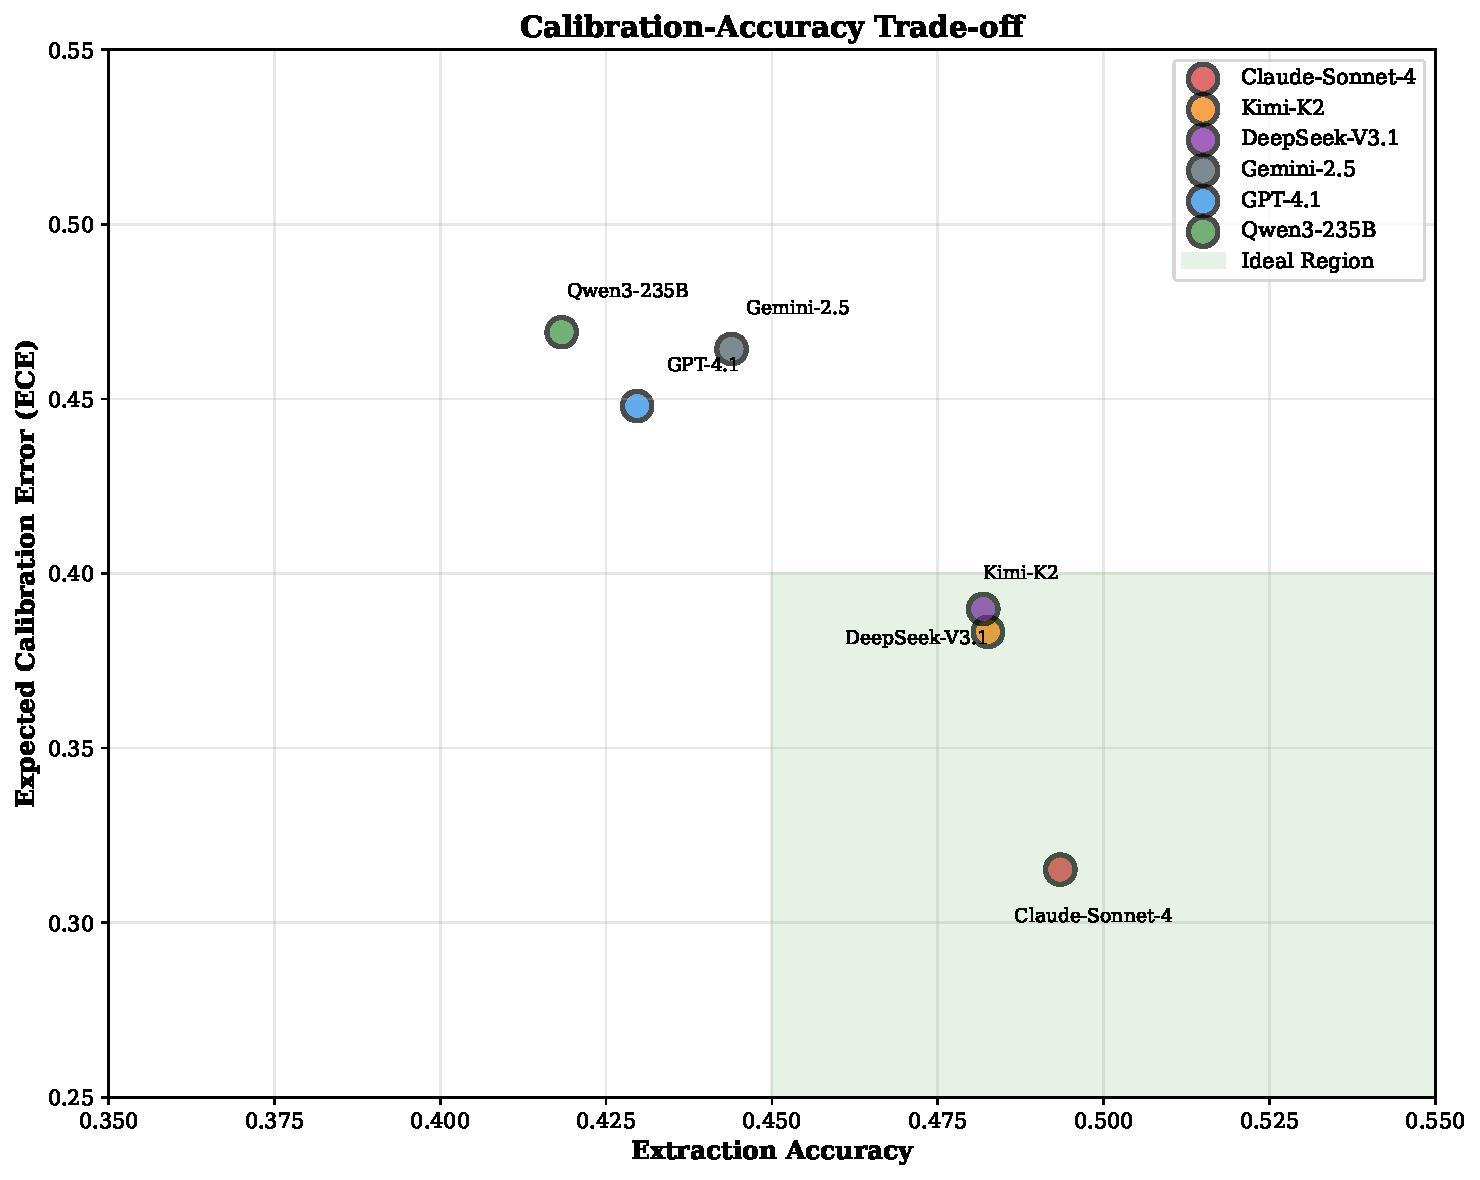
\includegraphics[width=0.8\linewidth]{fig_calibration_metrics.pdf}
  \caption{Accuracy-calibration trade-off. The green region indicates ideal performance (high accuracy, low ECE). \texttt{claude-sonnet-4} achieves the best balance with 49.3\% accuracy and 0.315 ECE.}
  \label{fig:calibration-tradeoff}
\end{figure}

% ============================================================================
% APPENDIX FIGURES (if space permits in main paper, otherwise move to appendix)
% ============================================================================

% PLACEMENT: Insert in Section 4.3 "Dataset-wise performance" (alternative view) OR Appendix A
% This provides a complementary visualization to fig_per_dataset_accuracy
\begin{figure}[htbp]
  \centering
  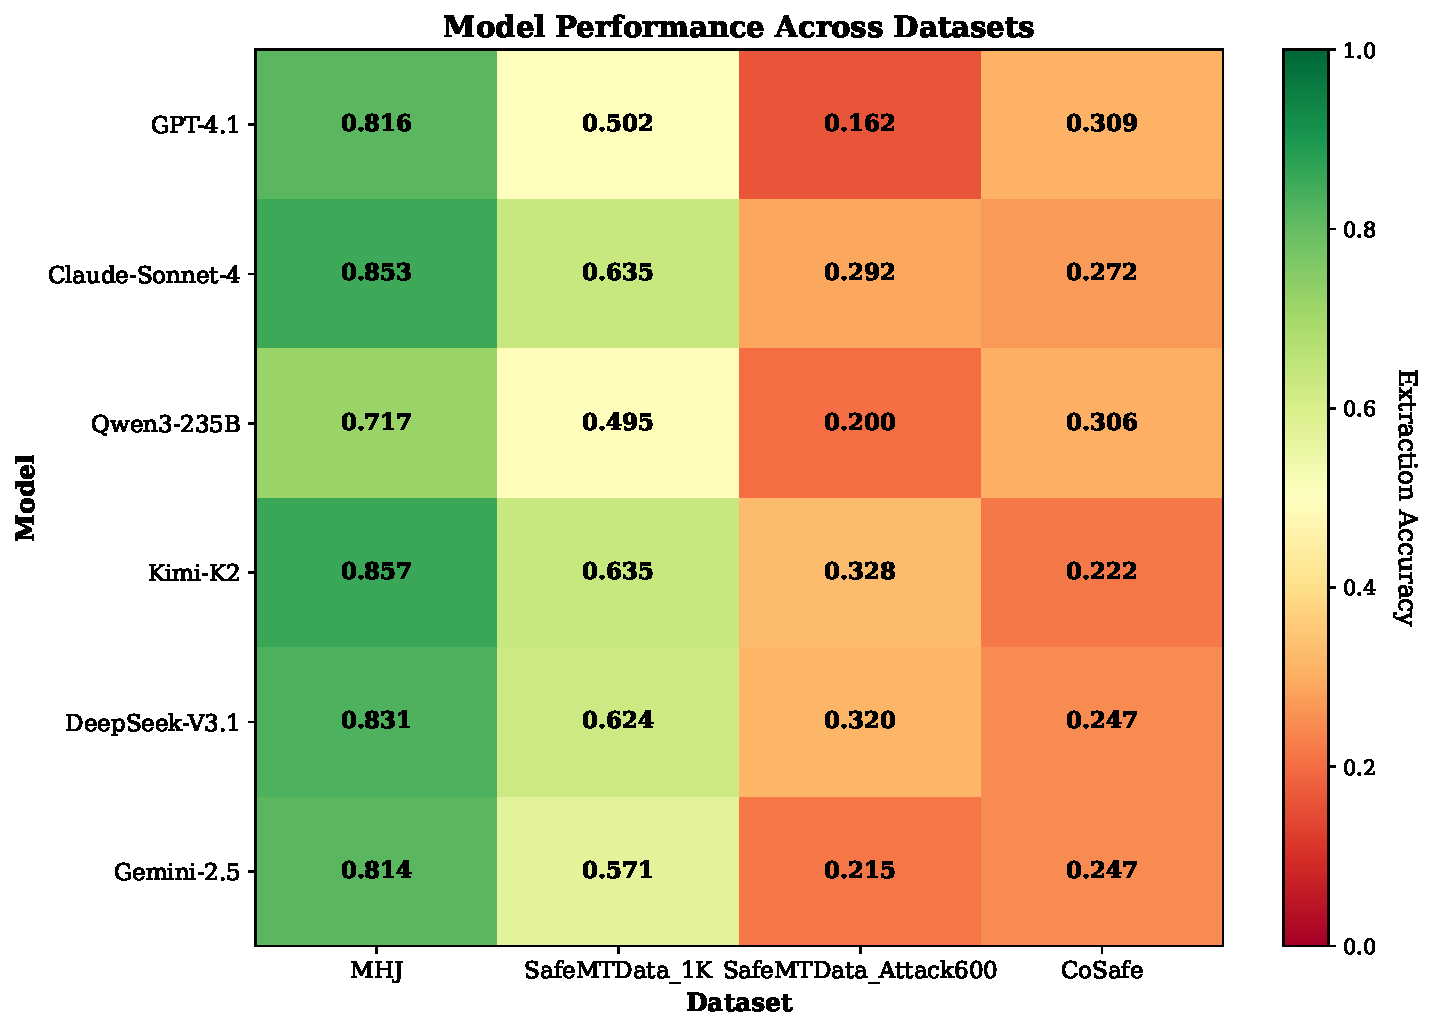
\includegraphics[width=\linewidth]{fig_dataset_heatmap.pdf}
  \caption{Heatmap visualization of model performance across datasets. Darker green indicates higher extraction accuracy. CoSafe consistently shows the strongest defense across all models.}
  \label{fig:dataset-heatmap}
\end{figure}

% PLACEMENT: Insert in Appendix A.10 "Confidence distributions"
% Detailed view of confidence distributions for calibration analysis
\begin{figure}[htbp]
  \centering
  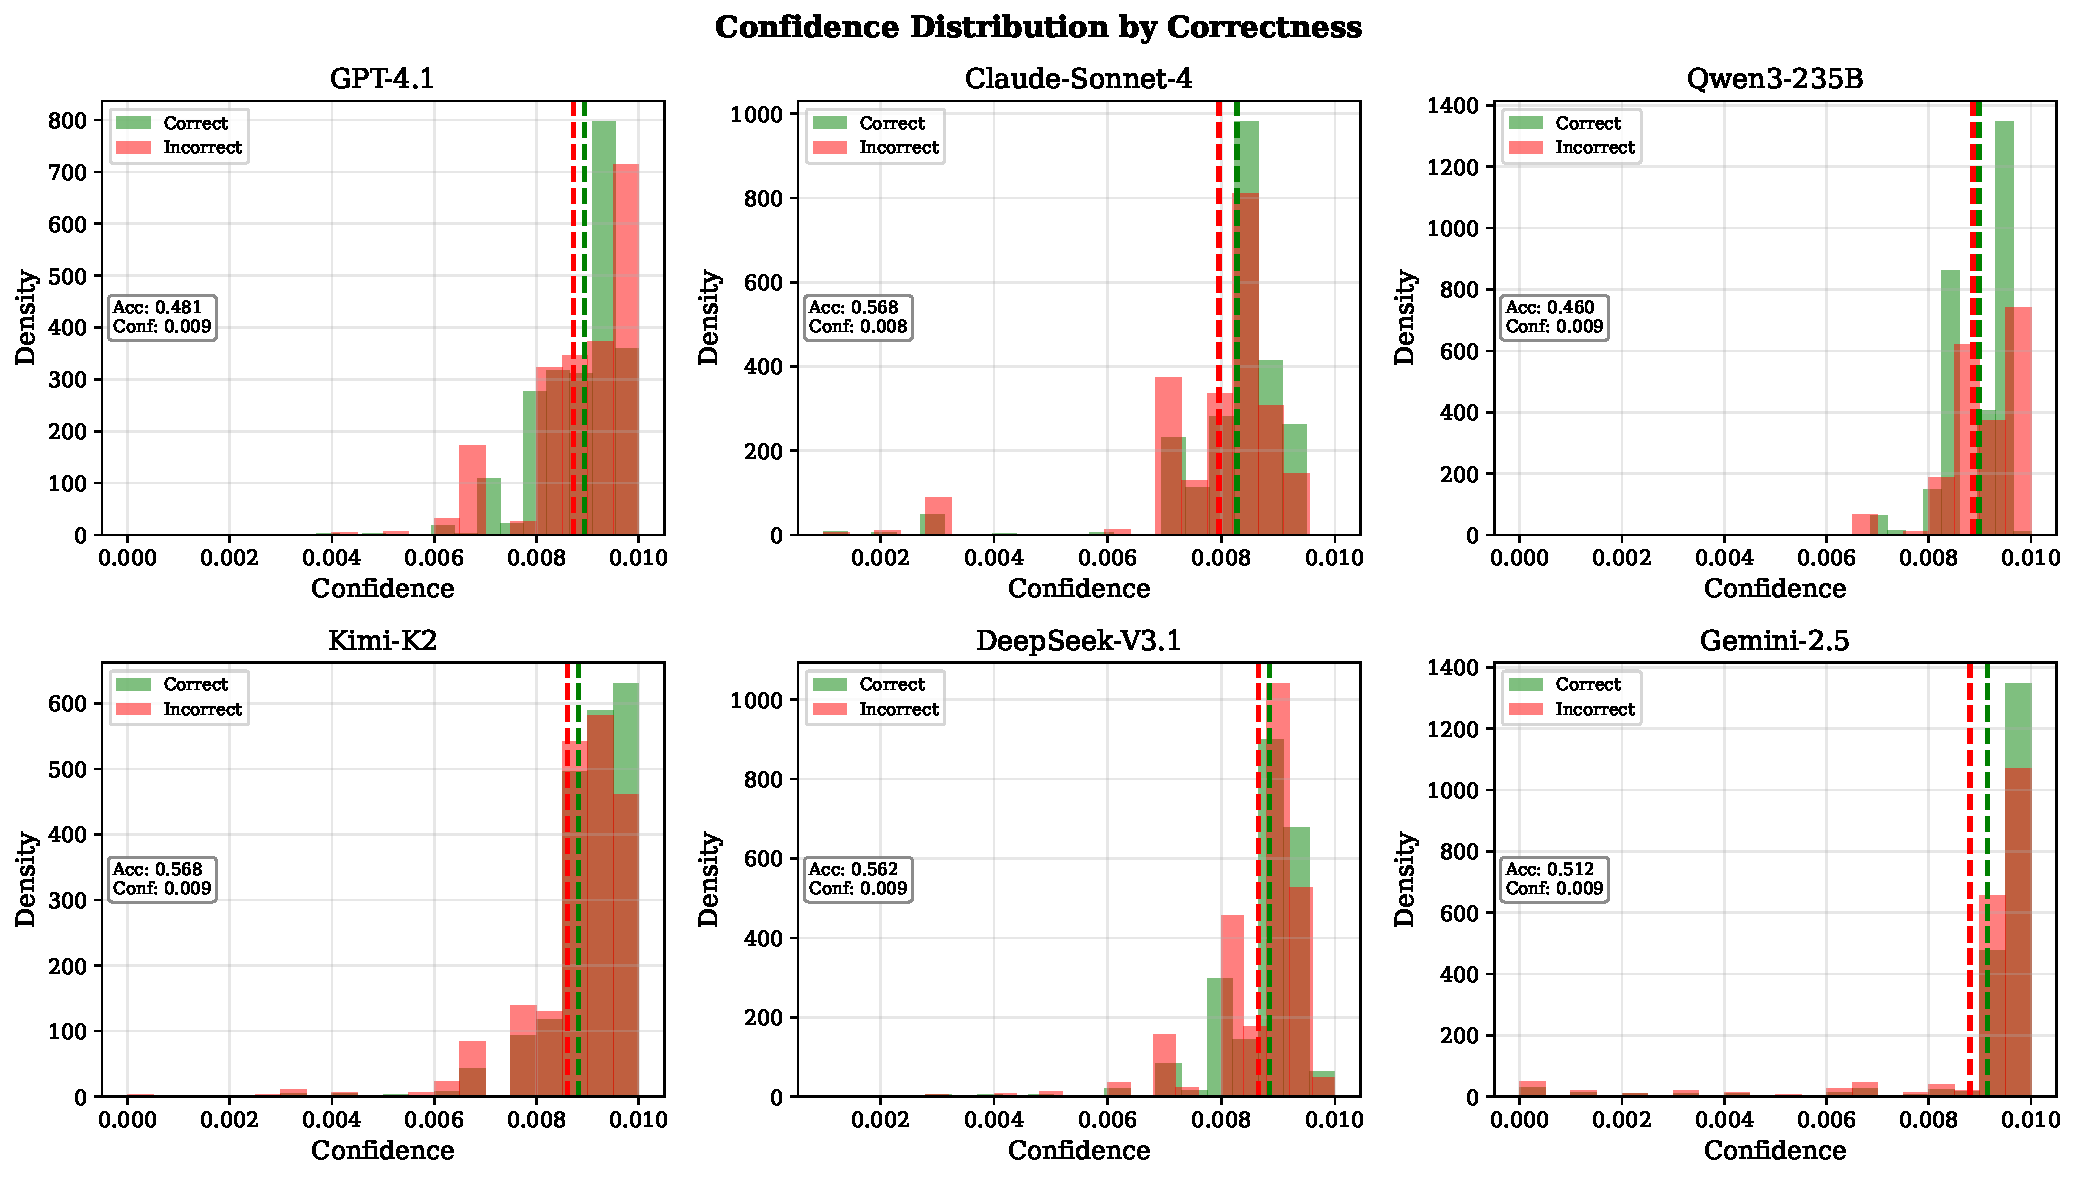
\includegraphics[width=\linewidth]{fig_confidence_distribution.pdf}
  \caption{Distribution of self-reported confidence scores for correct (green) and incorrect (red) extractions. Well-calibrated models like \texttt{claude-sonnet-4} show better separation between distributions.}
  \label{fig:confidence-distribution}
\end{figure}

% PLACEMENT: Insert in Section 4.4 "Metacognition" OR Appendix (if space limited)
% Comprehensive view of all metacognition metrics - can replace Table in main text
\begin{figure}[htbp]
  \centering
  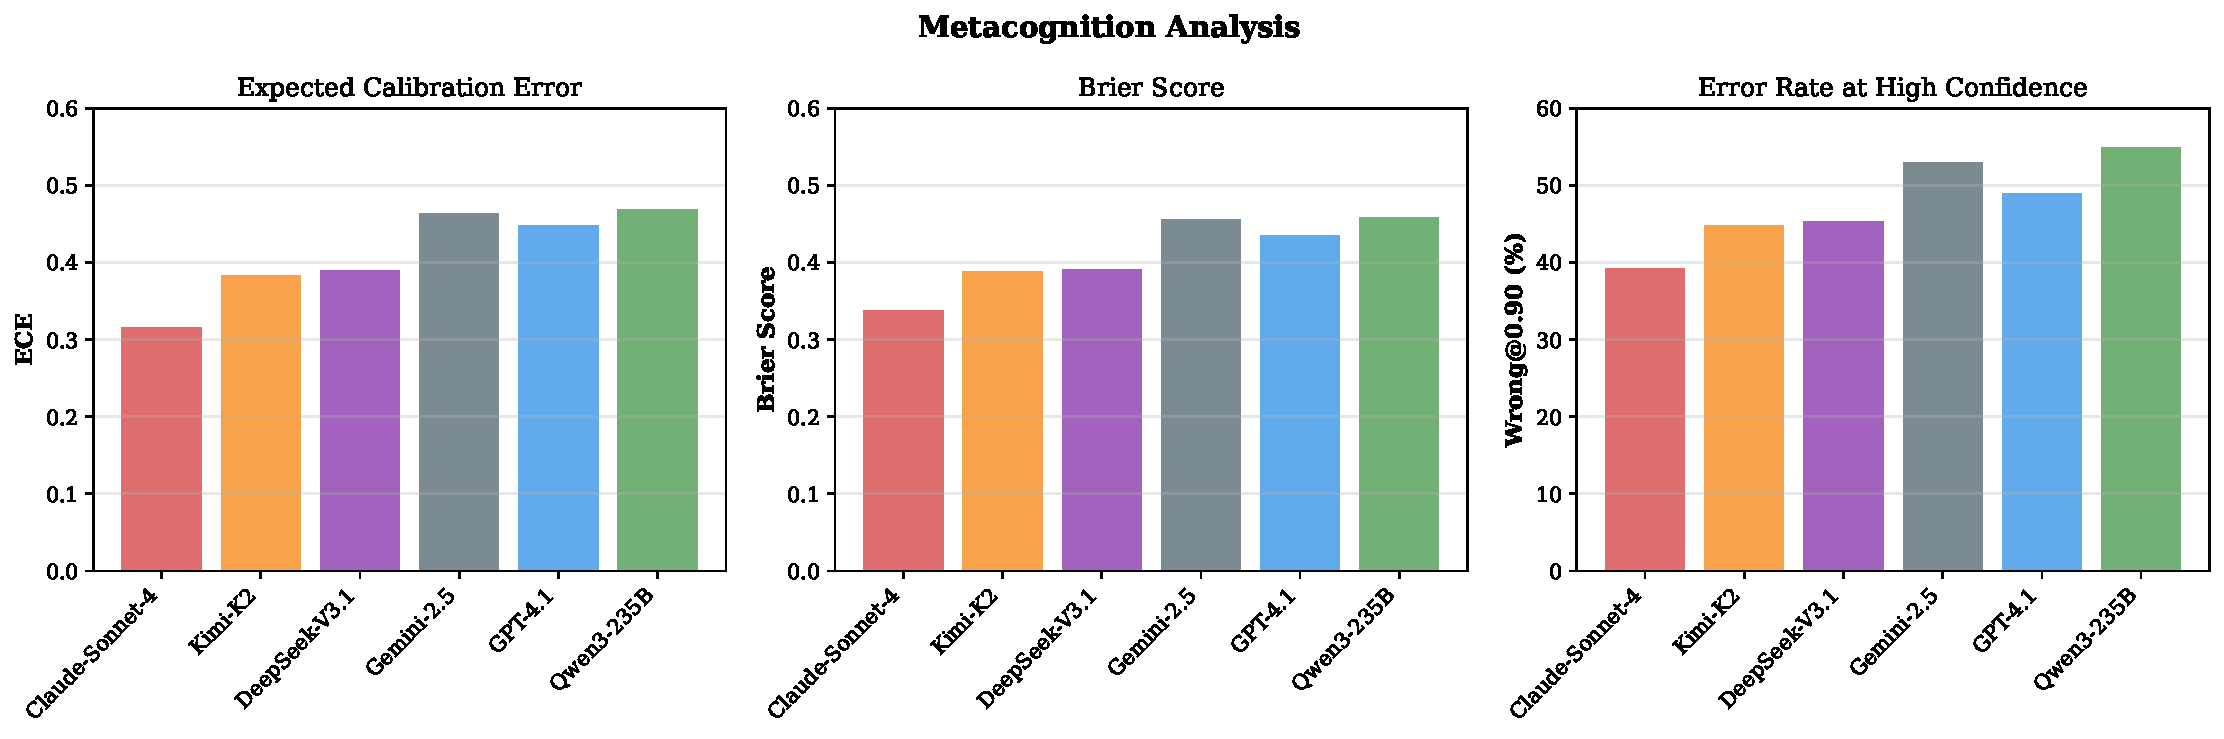
\includegraphics[width=\linewidth]{fig_metacognition.pdf}
  \caption{Metacognition metrics comparison: (a) Expected Calibration Error, (b) Brier Score, and (c) Wrong@0.90 (percentage of errors at $\geq$90\% confidence). Lower values indicate better calibration.}
  \label{fig:metacognition}
\end{figure}

% ============================================================================
% ALTERNATIVE COMPACT VERSION (if space is limited)
% ============================================================================

% PLACEMENT: Use this combined version in Section 4.4 if page limit is tight
% Combines fig_calibration_metrics and fig_confidence_distribution into one figure
% Option 1: Combine calibration figures
\begin{figure*}[t]
  \centering
  \subfloat[Accuracy vs ECE trade-off]{
    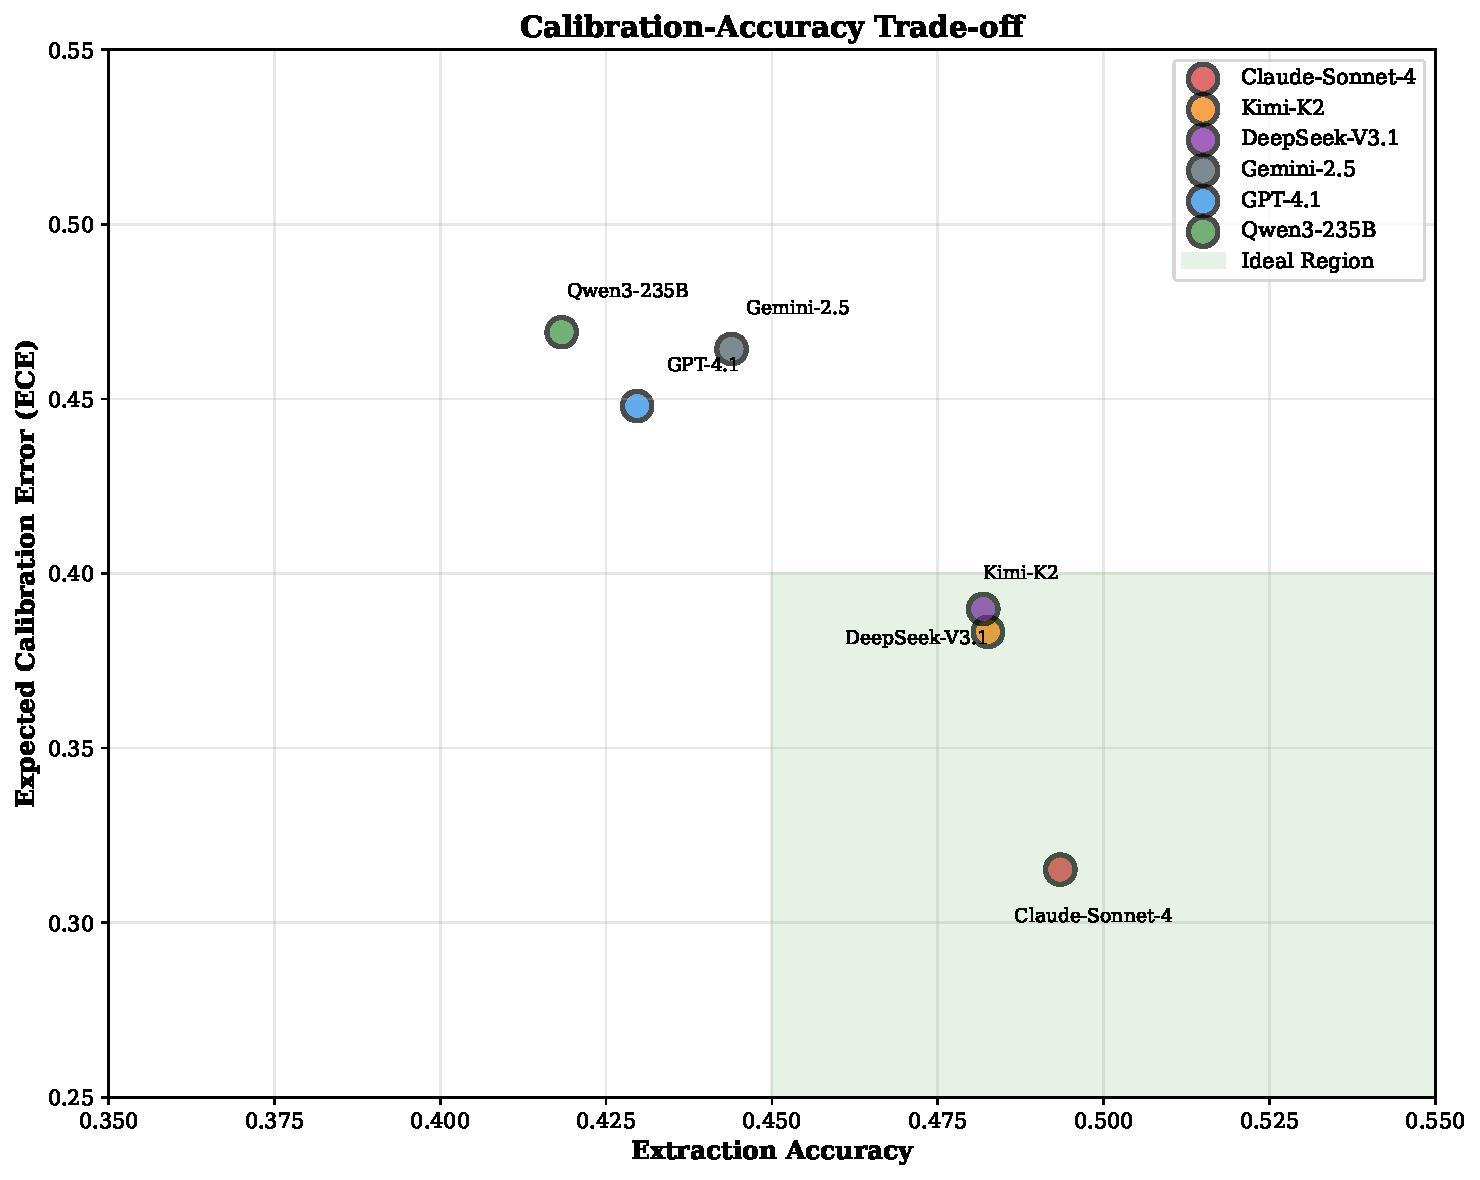
\includegraphics[width=0.48\linewidth]{fig_calibration_metrics.pdf}
  }
  \hfill
  \subfloat[Confidence distributions]{
    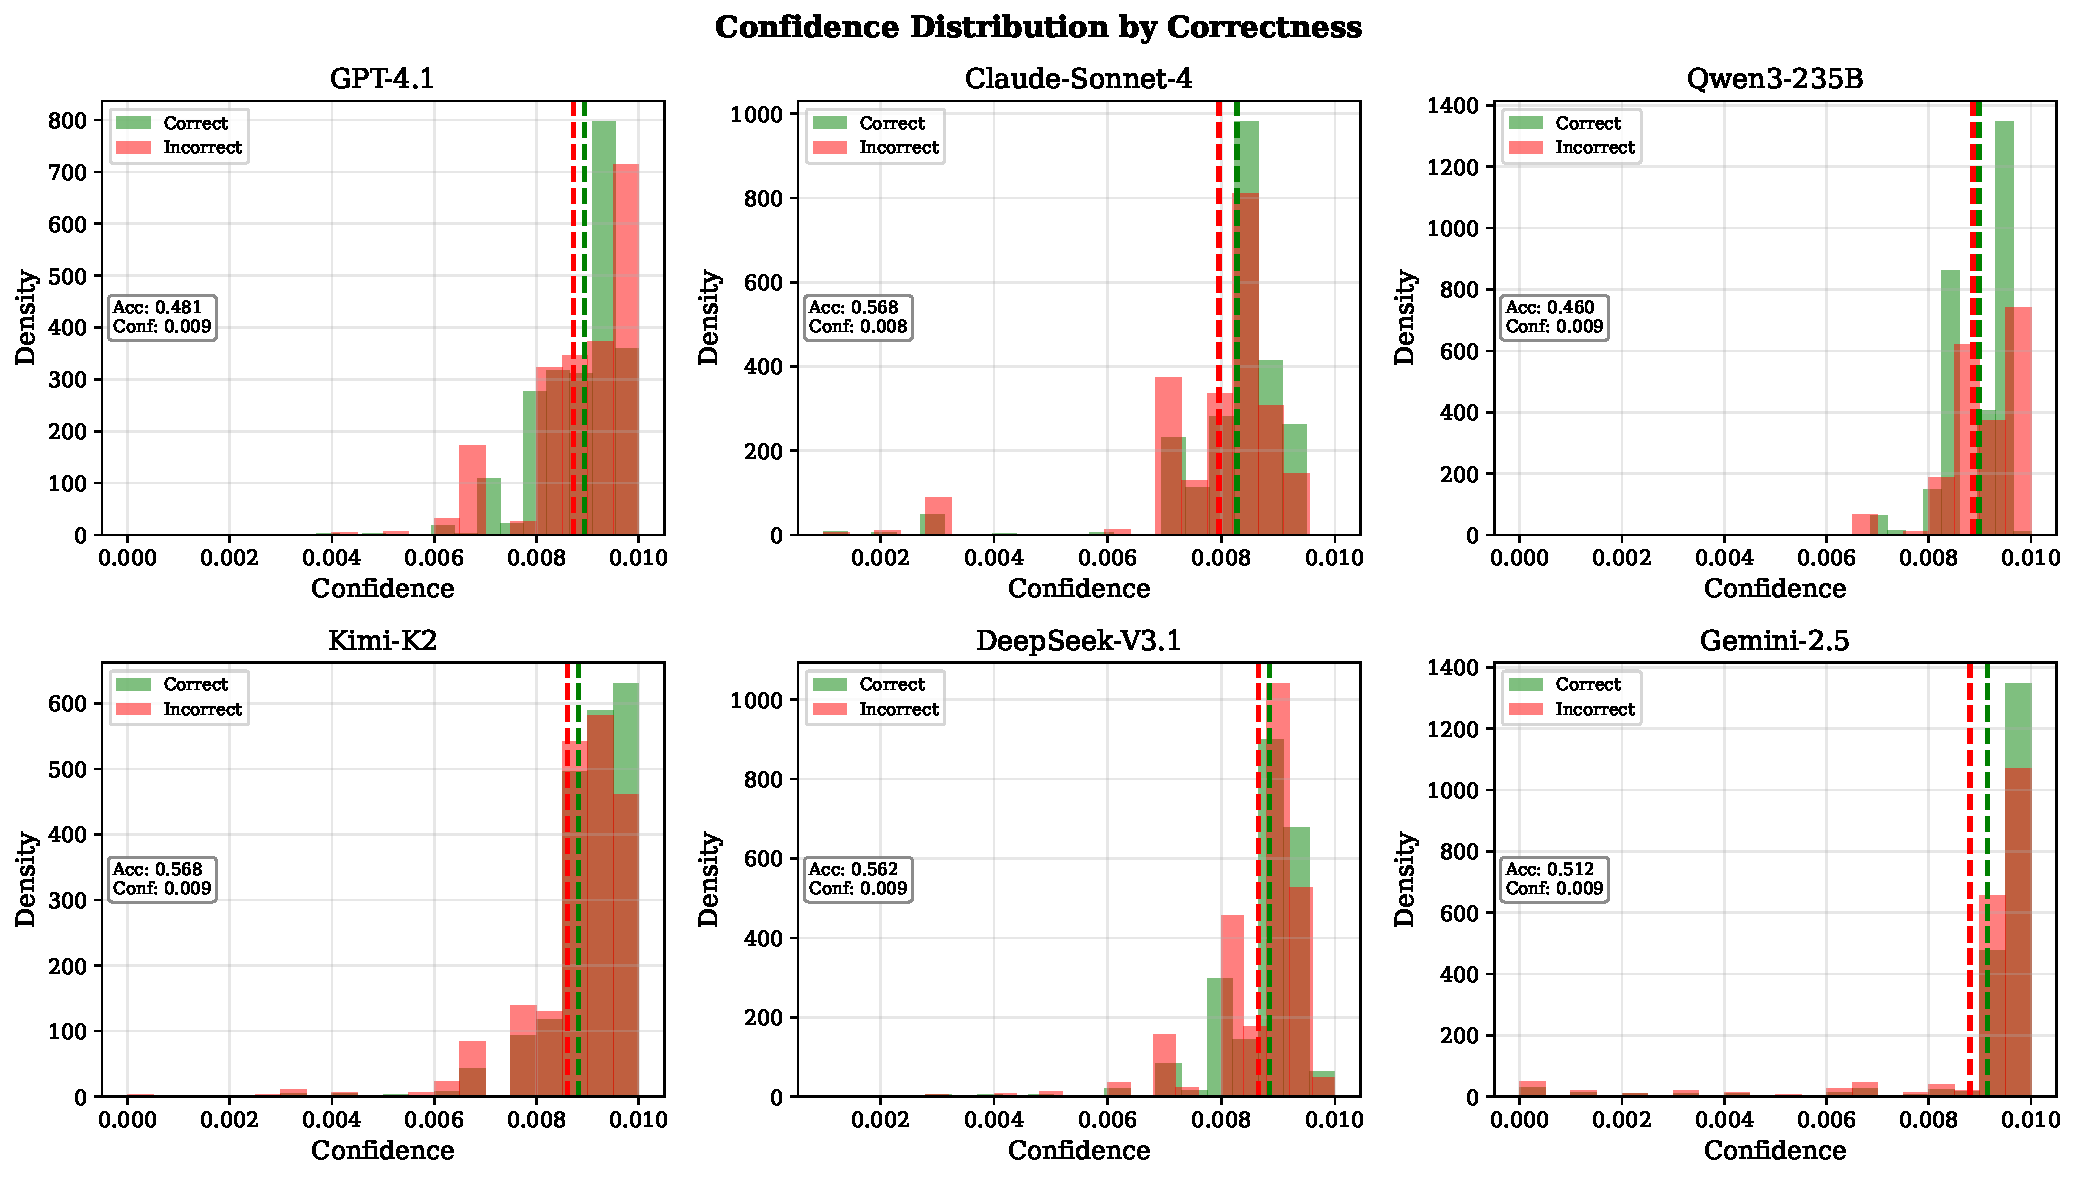
\includegraphics[width=0.48\linewidth]{fig_confidence_distribution.pdf}
  }
  \caption{Calibration analysis. (a) Models closer to bottom-right show better accuracy-calibration balance. (b) Separation between correct/incorrect confidence distributions indicates calibration quality.}
  \label{fig:calibration-combined}
\end{figure*}

% PLACEMENT: Use this combined version in Section 4.3 if page limit is tight
% Combines fig_per_dataset_accuracy and fig_dataset_heatmap for compact view
% Option 2: Combine dataset analysis figures
\begin{figure*}[t]
  \centering
  \subfloat[Bar chart comparison]{
    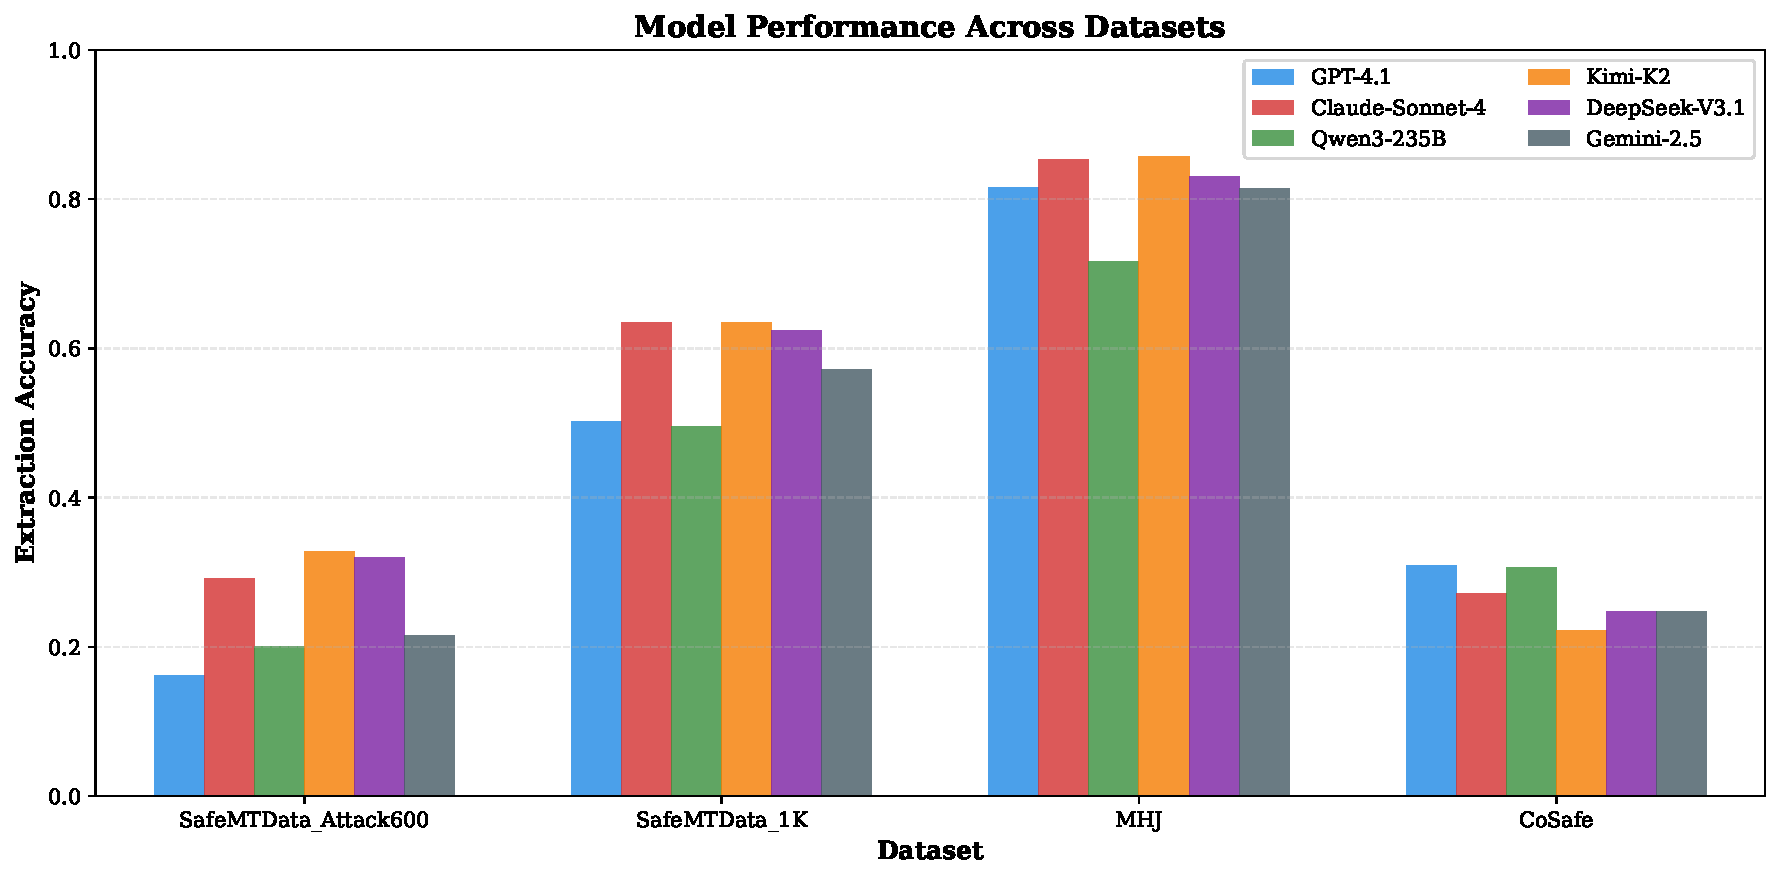
\includegraphics[width=0.48\linewidth]{fig_per_dataset_accuracy.pdf}
  }
  \hfill
  \subfloat[Heatmap visualization]{
    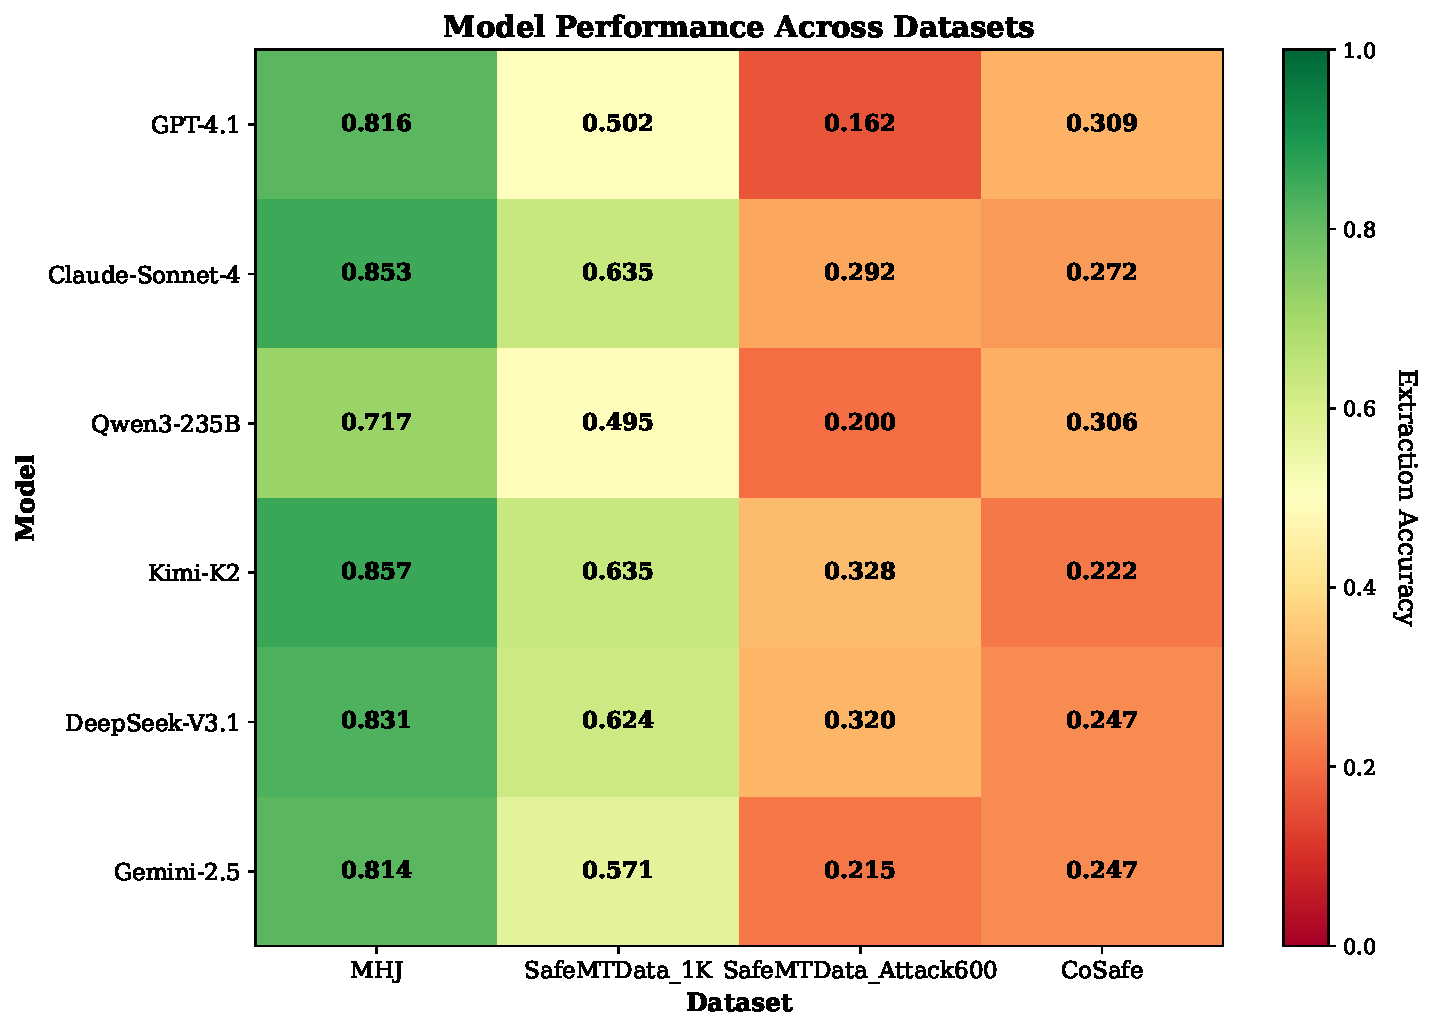
\includegraphics[width=0.48\linewidth]{fig_dataset_heatmap.pdf}
  }
  \caption{Model performance across datasets shown as (a) grouped bar chart and (b) heatmap. MHJ is easiest (mean 81.5\%), CoSafe is hardest (mean 25.7\%).}
  \label{fig:dataset-combined}
\end{figure*}

% ============================================================================
% SUMMARY TABLE TO ACCOMPANY FIGURES
% ============================================================================

% PLACEMENT: Insert in Section 4.2 or 4.4, depending on space and flow
% Can replace or supplement figure presentations of the same data
\begin{table}[t]
\centering
\caption{Summary of model performance on OBJEX dataset ($N{=}4,217$ per model, $\tau^*{=}0.66$).}
\label{tab:summary}
\begin{tabular}{lccccc}
\toprule
Model & Accuracy & 95\% CI & ECE$\downarrow$ & Wrong@0.9$\downarrow$ & AURC$\downarrow$ \\
\midrule
\texttt{claude-sonnet-4} & \textbf{0.493} & [0.479, 0.508] & \textbf{0.315} & \textbf{39.2\%} & \textbf{0.422} \\
\texttt{kimi-k2} & 0.483 & [0.468, 0.498] & 0.383 & 44.8\% & 0.434 \\
\texttt{deepseek-v3.1} & 0.482 & [0.467, 0.497] & 0.390 & 45.3\% & 0.444 \\
\texttt{gemini-2.5-flash} & 0.444 & [0.429, 0.459] & 0.464 & 53.0\% & 0.450 \\
\texttt{gpt-4.1} & 0.430 & [0.415, 0.445] & 0.448 & 48.9\% & 0.501 \\
\texttt{Qwen3-235B-A22B-FP8} & 0.418 & [0.403, 0.433] & 0.469 & 54.9\% & 0.524 \\
\bottomrule
\end{tabular}
\end{table>